\documentclass[11pt,a4paper,oneside]{article}
\usepackage{preamble}
\title{The Poset of Mesh Patterns}

\begin{document}
	\maketitle

%\section{Introduction}

\section{The Poset of Mesh Patterns}

Mesh patterns were first introduced in \cite{Bra11} and a concept of mesh
pattern containment was introduced in \cite{TU17}. A mesh pattern is of the form
$p=(\cl(p),\sh(p))$, where $\cl(p)$ is a permutation and $\sh(p)$ is a set of
coordinates corresponding to the boxes that are shaded, where $(i,j)$ denotes
the box $[i,i+1]\times[j,j+1]$, see \cref{fig:132}. We also denote $p$ by
$\cl(p)^{\sh(p)}$, for example $132^\emptyset$ is the mesh pattern on $132$ with
no shaded boxes. Let $G(p)$ be the set of coordinates of the points of $p$.

We let $|\cl(p)|$ represent the length of $\cl(p)$ and $|\sh(p)|$ the size of
$\sh(p)$, and define the length of $p$ as $|\cl(p)|$. We define the \emph{rank}
of $p$ as $|\pi|+|P|$, that is, the number of points plus the number of shaded
boxes.


\begin{figure}\centering\begin{tikzpicture}
\patt{1}{3}{1,3,2}[0/1,0/0,2/2][][][][][4]
\node (inv) at (0,-2){};
\end{tikzpicture}
\caption{The Mesh pattern $(132,\{(0,0),(0,1),(2,2)\})$, or equivalently $132^{(0,0),(0,1),(2,2)}$.}\label{fig:132}\end{figure}

Given two classical permutations $\sigma$ and $\pi$, an occurrence of $\sigma$
in $\pi$ is a map $\alpha:[|\sigma|]\rightarrow[|\pi|]$ such that
$\alpha(1)\alpha(2)\ldots\alpha(|\sigma|)$ has the same relative order of size
as $\sigma$. Given any letter $b=\sigma_i$ let
$\hat{\alpha}(b)=\pi_{\alpha(i)}$, so $\hat{\alpha}$ maps the value of a letter
in $\sigma$ to its value in $\pi$ under the map $\alpha$.

Using the notion of pattern occurrence we can define a partial order on
permutations where $\sigma\leP\pi$ if there is an occurrence of $\sigma$ in
$\pi$. Let $\mathcal{P}$ be the poset of all permutations with the partial order
$\leP$, we call this the \emph{classical permutation poset}.

We can extend this definition to define an occurrence in a mesh pattern.
Consider a pair of mesh patterns $m$ and $p$ and an occurrence $\alpha$ of
$\cl(m)$ in $\cl(p)$. Define
$R^\alpha_{i,j}=[\alpha(i),\alpha(i+1)]\times[\hat{\alpha}(j),\hat{\alpha}(j+1)]$,
this is the area in $p$ that corresponds to the box $(i,j)$ in $m$ according to
$\alpha$

An \emph{occurrence} of $m$ in $p$ is an occurrence $\alpha$ of $\cl(m)$ in
$\cl(p)$ satisfying $\bigcup_{(i,j)\in \sh(m)}R^\alpha_{i,j}\subseteq\sh(p)$ and
$G(p)\cap\bigcup_{(i,j)\in \sh(m)}R^\alpha_{i,j}=\emptyset$. This is equivalent
to saying every shaded point in $m$ corresponds to a fully shaded area in $p$
that contains no points.

\begin{figure}\centering
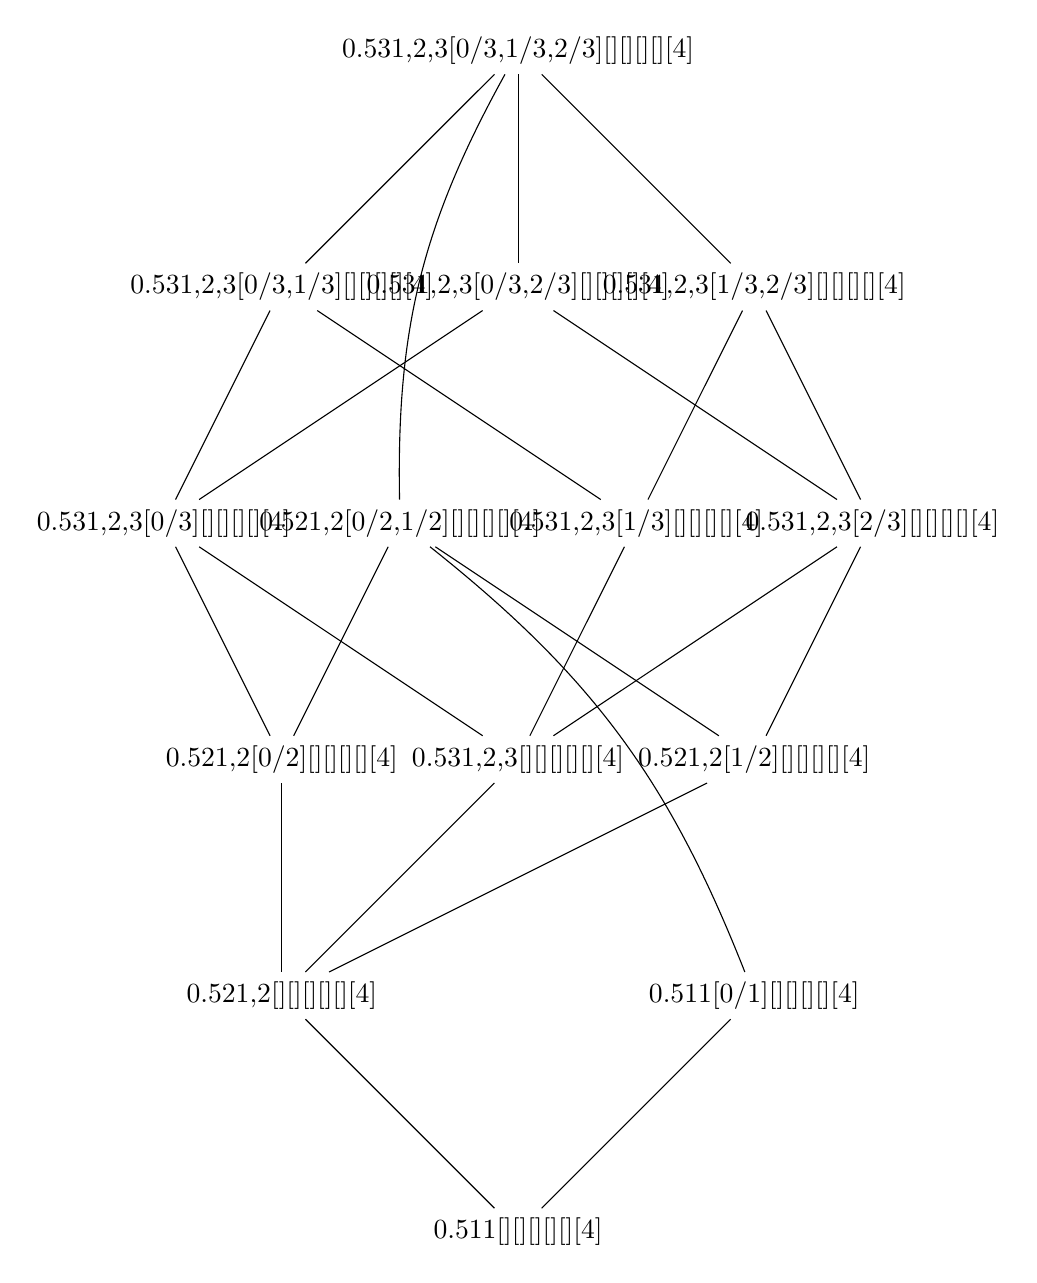
\begin{tikzpicture}
\def\y{3}
\def\x{3}
\def\s{0.5}
\node (123-123) at (0*\x,5*\y){\patt{\s}{3}{1,2,3}[0/3,1/3,2/3][][][][][4]};
\node (123-12) at (-1*\x,4*\y){\patt{\s}{3}{1,2,3}[0/3,1/3][][][][][4]};
\node (123-13) at (0*\x,4*\y){\patt{\s}{3}{1,2,3}[0/3,2/3][][][][][4]};
\node (123-23) at (1*\x,4*\y){\patt{\s}{3}{1,2,3}[1/3,2/3][][][][][4]};
\node (123-1) at (-1.5*\x,3*\y){\patt{\s}{3}{1,2,3}[0/3][][][][][4]};
\node (12-12) at (-0.5*\x,3*\y){\patt{\s}{2}{1,2}[0/2,1/2][][][][][4]};
\node (123-2) at (0.5*\x,3*\y){\patt{\s}{3}{1,2,3}[1/3][][][][][4]};
\node (123-3) at (1.5*\x,3*\y){\patt{\s}{3}{1,2,3}[2/3][][][][][4]};
\node (12-1) at (-1*\x,2*\y){\patt{\s}{2}{1,2}[0/2][][][][][4]};
\node (123-0) at (0*\x,2*\y){\patt{\s}{3}{1,2,3}[][][][][][4]};
\node (12-2) at (1*\x,2*\y){\patt{\s}{2}{1,2}[1/2][][][][][4]};
\node (12-0) at (-1*\x,1*\y){\patt{\s}{2}{1,2}[][][][][][4]};
\node (1-1) at (1*\x,1*\y){\patt{\s}{1}{1}[0/1][][][][][4]};
\node (1-0) at (0*\x,0*\y){\patt{\s}{1}{1}[][][][][][4]};
\draw (123-123) -- (123-12);\draw (123-123) -- (123-13);\draw (123-123) -- (123-23);
\draw[-] (123-123) to [bend right=15] (12-12);\draw[-] (12-12) to [bend left=15] (1-1);
\draw (123-12) -- (123-1);\draw (123-12) -- (123-2);
\draw (123-13) -- (123-1);\draw (123-13) -- (123-3);
\draw (123-23) -- (123-2);\draw (123-23) -- (123-3);
\draw (123-1) -- (123-0);\draw (123-1) -- (12-1);
\draw (123-2) -- (123-0);
\draw (123-3) -- (123-0);\draw (123-3) -- (12-2);
\draw (12-12) -- (12-1);\draw (12-12) -- (12-2);
\draw (12-1) -- (12-0);\draw (12-2) -- (12-0);
\draw (123-0) -- (12-0);\draw (12-0) -- (1-0);
\draw (1-1) -- (1-0);
\end{tikzpicture}
\caption{The interval $[1^\emptyset,123^{(0,3),(1,3),(2,3)}]$ of $\mathcal{M}$.}\label{fig:intEx}
\end{figure}

\section{M\"obius Function}
We begin with some simple results we can immediately deduce about this poset.
First we consider the case that two mesh patterns have the same underlying permutation.

\begin{lem}
If $\cl(m)=\cl(p)$, then $[m,p]$ is isomorphic to the boolean lattice
$B_{|\sh(p)|-|\sh(m)|}$ which implies $\mu(m,p)=(-1)^|\sh(p)|-|\sh(m)|$ and
$[m,p]$ is shellable.
\begin{proof}
We cannot remove any points from $p$, we can only unshade boxes, and we can
unshaded any boxes from $\sh(p)\setminus\sh(s)$ in any order.
\end{proof}
\end{lem}

The simplest mesh patterns are those with no points, that is, the mesh patterns
with a single box that is shaded or unshaded, which we denote
$\epsilon^\emptyset$ and $\epsilon^{(0,0)}$, respectively.

\begin{lem}
Consider a mesh pattern $p$, then:
$$\mu(\epsilon^{A},p)=\begin{cases}
1,&\mbox{ if }p=\epsilon^A \\
-1,&\mbox{ if }A=\emptyset\,\,\&\,\,\rk(p)=1\\
0,&\mbox{ otherwise}
\end{cases}$$
\begin{proof}
The cases $p=\epsilon^A$ and $A=\emptyset\,\,\&\,\,\rk(p)=1$ are trivial. The
mesh pattern $\epsilon^{(0,0)}$ is not contained in any large mesh patterns, so
the M\"obius function is always $0$. If $\rk(p)>1$, then
$(\epsilon^\emptyset,p)$ contains a unique minimal element $1^\emptyset$, so
$\mu(\epsilon^\emptyset,p)$.
\end{proof}
\end{lem}

If two mesh patterns have no shadings then we have an interval from the
classical poset.

\begin{lem}
If $\sh(s)=\sh(p)=\emptyset$, then $[s,p]$ is isomorphic to the interval
$[\cl(s),\cl(p)]$ in $\mathcal{P}$, so $\muM(s,p)=\muP(\cl(s),\cl(p))$.
\end{lem}
The M\"obius function of the classical permutation poset is known to be
unbounded \cite{Smith13}. So we get the following corollary:

\begin{cor}
The M\"obius function is unbounded on $\mathcal{M}$.
\end{cor}

We can also show that the M\"obius function is unbounded if we include shadings.

\begin{lem}\label{lem:mobUn}
Let $m$ be a mesh pattern with exactly one descent, where the descent bottom is
the letter $1$, and all boxes south west of the point $1$ are shaded, then
$$\mu(21^{(0,0),(1,0)},m)=\begin{cases}
(-1)^{|m|}\lfloor\frac{n}{2}\rfloor,&\mbox{ if } \cl(m) \mbox{ has no adjacencies}\\
1,&\substack{ \text{ if } \cl(m) \text{ has exactly one letter before the descent} \\\text{ in an adjacency tail and none after}}\\
0, &\mbox{ otherwise}
\end{cases}$$
Moreover, $[21^{(0,0),(1,0)},m]$ is shellable.
\begin{proof}
Note that every mesh pattern in $I=[21^{(0,0),(1,0)},m]$ has exactly one descent
and everything SW of the point $1$ shaded. Define a bijection $f$ from $I$ to
the poset of words with subword order where the $i-1$'th letter of $f(p)$ is $0$
if $i$ is before the letter $1$ in $p$ and $1$ if after the letter $1$, for all
$1<i\le n$. So $21^{(0,0),(1,0)}$ maps to the word $0$. A mesh pattern in $I$ is
uniquely determined by the value of the points before the descent, because these
values must appear first followed by the letter $1$ and then the remaining
letters. Therefore, it is straightforward to see this is a bijection and to
check that it is order preserving. So $I$ is isomorphic to an interval of the
poset of words with subword order. It was shown in \cite{Bjo90} that these
intervals are shellable and the M\"obius function equals the number of normal
occurrences, where an occurrence is normal if in any run of equal elements every
non-initial letter is part of the occurrence, which implies the result.
\end{proof}
\end{lem}

We can also see that the M\"obius function on $\mathcal{M}$ is not bounded the
classical poset, that is, it is not true that $\muM(m,p)\le
\muP(\cl(m),\cl(p))$. A simple counterexample is the interval
$[1^{(0,1)},123^{(0,2),(0,3),(1,2),(1,3)}]$, this has M\"obius number $1$,
however $\muP(1,123)=0$.

If we consider intervals where the bottom mesh pattern has no shadings, then we
get the following result:

\begin{lem}\label{lem:mu0}
Consider the interval $[m,p]$ in $\mathcal{M}$. If $\sh(m)=emptyset\not=\sh(p)$
and there is no $s\in(m,p)$ with $\cl(s)=\cl(m)$, then $\mu(m,p)=0$.
\begin{proof}
Define a map $f(x)=\cl(x)^\emptyset$, for any $x\in(m,p)$. Let $A$
order-preserving image $f((m,p))$. Note that $\mu(A)$ is contractible because it
has a unique maximal element $\cl(p)^\emptyset$. Moreover, for any $y\in A$
$f^{-1}(A_{\ge y})$ equals $[y,p)$ which is contractible. Therefore, $(m,p)$ is
homotopically equivalent to $A$ using the Quillen Fiber Lemma, which implies
$\mu(m,p)=0$. This is also called a retraction.
\end{proof}
\end{lem}
We can combine Lemma~\ref{lem:mu0} with he following result to see that the
M\"obius function is almost always zero on the interval $[1^\emptyset,p]$.
\begin{lem}
As $n$ tends to infinity the proportion of permutations that contain one of
$\{1^{(0,0)},1^{(1,0)},1^{(0,1)},1^{(1,1)}\}$ approaches $0$.
\begin{proof}
Let $P(n,i)$ be the probability that the letter $i$ is an occurrence of
$1^{(0,0)}$ in a length $n$ mesh pattern. And let $P(n)$ be the probability that
a length $n$ mesh pattern contains $1^{(0,0)}$.

The probability that $i$ is an occurrence of $1^{(0,0)}$ is given by selecting
the location $k$ of $i$, each has probability $\frac{1}{n}$, and then we require
that all boxes south west of $i$ are filled, of which there are $2^{ik}$. Note
that this over estimates the probability, because it is possible that there is a
point south west of $i$, which would imply $i$ is not an occurrence of
$1^{(0,0)}$, however this argument still counts them. We can formulate this as:

\begin{align*}
P(n,i)&\le\sum_{k=1}^{n+1-i}\frac{1}{n}\left(\frac{1}{2^i}\right)^k=\frac{1}{n}\left(\frac{2^{-i(n+2-i)}}{2^{-i}-1}-1\right)=\frac{1}{n2^i}\left(\frac{1-2^{-i(n+1-i)}}{1-2^{-i}}\right)\le\frac{2}{n2^i}
\end{align*}

To compute the probability that a length $n$ permutation contains $1^{(0,0)}$ we
can sum over all letters $i$ and test if $i$ is an occurrence of $1^{(0,0)}$.
Note again this is an over estimate because if a permutation contains multiple
occurrences of $1^{(0,0)}$ it counts that permutation more than once.

$$P(n)\le\sum_{i=1}^{n}P(n,i)\le\sum_{i=1}^{n}\frac{2}{n2^i}=\frac{2}{n}\left(\frac{\left(\frac{1}{2}\right)^{n+1}-1}{\frac{1}{2}-1}-1\right)\le\frac{2}{n} $$

We can repeat this calculation for the other three one shadings of $1$ so we get
that $P(n)\le \frac{4}{n}\rightarrow 0$.
\end{proof}
\end{lem}
\begin{cor}
As $n$ tends to infinity the proportion of mesh patterns $p$ of length n such
that $\mu(1^\emptyset,p)=0$ approaches $1$.
\end{cor}

In the classical case it is true that given a permutation $\sigma$ the
probability a permutation of length $n$ contains $\sigma$ tends to $1$ as $n$
tends to infinity, this follows from the Marcus-Tardos Theorem \cite{MT04}. By
the above result we can see the same is not true in the mesh pattern case. In
fact we conjecture the opposite is true:

\begin{conj}
Given a mesh pattern $m$, the probability that a random mesh pattern of length
$n$ contains $m$ tends to $0$ as $n$ tends to infinity.
\end{conj}




\section{Purity}

Interestingly the mesh pattern poset is not a pure poset, that is, not every
maximal chain has the same length. We say an edge $x\lessdot y$ is \emph{impure}
if $\rk(y)-\rk(x)>1$. Let $m-p$ be the mesh pattern obtained by deleting the
point $p$ and let $m\setminus p$ be the occurrence of $m-p$ in $m$. We say that
deleting a point $p$ \emph{merges shadings} if there is a shaded box in $m-p$
that corresponds to more than $1$ shaded box in $m\setminus p$.

\begin{lem}\label{lem:impureEdge}
An edge between $x\lessdot y$ is impure if and only if all occurrences of $x$ in
$y$ use all shaded boxes of $y$ and are obtained by deleting a point that merges
shading.
\begin{proof}
First we show the backwards direction. Because $x$ is obtained by deleting a
point that merges shadings $x$ must have one less point and at least one less
shading so $\rk(y)-\rk(x)\ge2$. So it suffices to show that there is no $z$ such
that $x<z<y$. Suppose such a $z$ exists, then if $z$ is obtained by deshading a
box in $y$ it can no longer contain $x$ because all occurrences of $x$ in $y$
use all shaded areas of $y$. If $z$ is obtained by deleting a point, then that
cannot remove shadings, only merge shadings, otherwise it wouldn't contain $x$,
and it implies $cl(x)=cl(z)$. Moreover, if $x<z$ then we can deshade some boxes
of $z$ to get $x$ which implies there is an occurrence of $x$ in $y$ that
doesn't use all the shaded boxes of $y$.

Now consider the forwards direction, so suppose $x\lessdot y$ is impure. So
$\rk(y)-\rk(x)\ge2$, which implies $x$ is obtained by deleting a single point
which merges shadings but does not delete shadings, because any other
combination of deleting points and deshading can be done in successive steps.
Furthermore, this must be true for any point that can be deleted to get $x$,
that is, for all occurrences of $x$ in $y$. Moreover, if there is an occurrence
that doesn't use all the shaded boxes of $y$, we can deshade the box it doesn't
use and get an element that lies between $x$ and $y$.
\end{proof}
\end{lem}

\begin{lem}\label{lem:topImpure}
If there is an impure edge in $[1^\emptyset,m]$, then there is an impure edge
$a\lessdot b$ where $cl(m)=cl(b)$.
\begin{proof}
If $x\lessdot y$ is an impure edge in $[1^\emptyset,m]$, then let $b$ be a mesh
pattern obtained by adding points to $y$ to get the classical pattern $b$. Pick
an occurrence of $x$ in $y$ and add the points to $x$ in the order induced by
how they are added to $y$ and the occurrence, call this $a$. The points added
will not have any shadings in the four boxes touching it, therefore no point
touching a shading in $a$ can embed in a new point of $b$. Moreover, the set of
embeddings of $a$ in $b$ is a subset of $x$ in $y$, after adding the new points
to each. These two conditions imply that if every embedding of $x$ in $y$ uses
all the shadings of $y$, this is also true for every embedding of $a$ in $b$.
Therefore, the result follows by Lemma~\ref{lem:impureEdge}.
\end{proof}
\end{lem}

\begin{prop}
Consider a mesh pattern $m$. The interval $[1^\emptyset,m]$ is non-pure if and
only if there exists a point $p$ in $m$ such that $m-p$ merges shadings and
there is no other occurrence of $m-p$ in $m$ with a subset of shadings of
$m\setminus p$.
\begin{proof}
First we show the backwards direction. Let $x$  be the mesh pattern obtained by
inserting $p$ back into $m^p$, and $\eta$ the corresponding embedding of $m^p$
in $x$. Note that it is not always true that $x=m$ because some shaded shadings
of $m$ are lost when deleting $p$. We claim that $m^p\lessdot x$ is an impure
edge. This follows by Lemma~\ref{lem:impureEdge} because by $\eta$ uses all the
shaded boxes in $x$ and there is no subshading occurrence.

To see the other direction suppose there is an impure edge in $[\omega,m]$. By
Lemma~\ref{lem:topImpure} there is an impure edge $a\lessdot b$ where
$cl(b)=cl(m)$. If $m$ is impure then it must remove both a point and a shading,
so it must merge shadings by deleting some point $p$ and there is no element
between them so there can be no subshading of $b$ that contains $a$.
\end{proof}
\end{prop}

\begin{cor}
There is an impure edge in the interval $[m,p]$ if and only if there exists a
point $x$ in $p$ such that $p-x$ merges shadings and there is no other
occurrence of $p-x$ in $p$ with a subset of shadings of $p\setminus x$, and
$p-x\ge m$.
\end{cor}

Note that containing an impure edge in $[m,p]$ does not necessarily imply there
that $[m,p]$ is non-pure. For example, if $[m,p]$ contains only one edge and
that edge is impure, then $[m,p]$ is still pure. So it is necessary that there
is an impure edge and a pure edge in the interval. Although it is also possible
to have an non-pure poset that only contains impure edges, if the difference
between the ranks of the elements at ends of the edges varies.


\section{Topology}

If $[\cl(s),\cl(p)]$ is (dis)connected in $\mathcal{P}$ it does no imply $[s,p]$
has the same property in $\mathcal{M}$. For example, the interval $[123,456123]$
is disconnected in the classical permutation poset but in $\mathcal{M}$ the
interval $[123^{(3,0),(3,1),(3,2)},456123^{(6,0),(6,1),(6,2)}]$, see
\cref{fig:123}, is chain, so is connected. Furthermore, the interval
$[321,521643]$ is connected in $\mathcal{P}$ but $[321^{(1, 3)},521643^{(1, 5),
(1, 6), (4, 6)}]$, see \cref{fig:321}, is disconnected in $\mathcal{M}$.

\begin{figure}[h]\centering
\patt{.5}{3}{1,2,3}[3/0,3/1,3/2][][][][][4]
\patt{.5}{6}{4,5,6,1,2,3}[6/0,6/1,6/2][][][][][4]
\caption{The mesh patterns $123^{(3,0),(3,1),(3,2)}$ and $456123^{(6,0),(6,1),(6,2)}$}\label{fig:123}
\end{figure}
\begin{figure}[h]\centering
\patt{.5}{3}{3,2,1}[1/3][][][][][4]
\patt{.5}{6}{5,2,1,6,4,3}[1/5,1/6,4/6][][][][][4]
\caption{The mesh patterns $321^{(1, 3)}$ and $521643^{(1, 5), (1, 6), (4, 6)}$}\label{fig:321}
\end{figure}

This also implies that if $[\cl(s),\cl(p)]$ is (non-)shellable in $\mathcal{P}$
then it is not true that $[s,p]$ has the same property in $\mathcal{M}$. This
follows by the previous examples, $[123,456123]$ is not shellable but
$[123^{(3,0),(3,1),(3,2)},456123^{(6,0),(6,1),(6,2)}]$ is shellable, and
$[321,521643]$ is shellable but $[321^{(1, 3)},521643^{(1, 5), (1, 6), (4, 6)}]$
is not shellable.

We can define a direct sum operation on mesh patterns, where given two mesh
patterns $s$ and $t$, where the top right corner of $s$ and bottom left corner
of $t$ are not shaded, the direct sum $s\oplus t$ has classical pattern
$\cl(s)\oplus\cl(t)$ and the shadings are given by placing $t$ north east of $s$
and shading any borders so they extend to the edge. We can similarly define the
skew-sum.

\begin{lem}
If $m$ is indecomposable and $(0,0),(|m|,|m|)\not\in\sh(m)$, then
$[m,m\oplus m]$ is disconnected.
\begin{proof}
There are exactly two occurrences of $m$ in $m\oplus m$, the first $|m|$ letters
$\eta_1$ or the last $|m|$ letters $\eta_2$. If you delete a point or deshade
any box that is not in $\eta_1$ then that point or box must be part of $\eta_2$,
so the resulting mesh pattern only contains one occurrence of $m$ which
corresponds to $\eta_1$ so then you can only delete points or shadings that are
not part of $\eta_1$ so must be part of $\eta_2$. A similar argument applies if
you initial delete a point or shading not part of $\eta_2$. Therefore, any two
points/shading removals must both be part of $\eta_1$ or $\eta_2$, thus the
poset can be split into components where on one side we remove elements not in
$\eta_1$ and the other elements not in $\eta_2$.
\end{proof}
\end{lem}
\begin{cor}
If $m$ is indecomposable and $(|m|,0),(0,|m|)\not\in\sh(m)$, then
$[m,m\ominus m]$ is disconnected.
\end{cor}

A analogous result is used in the classical case in \cite{McSt13} to show that
almost all intervals of the classical permutation poset are not shellable. The
proof of this follows form the Marcus-Tardos theorem, we have seen this result
does not apply in the mesh pattern case so we cannot prove a similar result
using this technique.  A similar problem was studied for boxed mesh patterns in
permutations in \cite{AKV13}, which is equivalent to boxed mesh patterns in
fully shaded mesh patterns. So we leave it as an open question:

\begin{que}
What proportion of intervals of $\mathcal{M}$ are shellable?
\end{que}


\bibliographystyle{alpha}
\bibliography{bibfile}
\end{document}
